Na testovanie mobilnej aplikácie bolo zachytených 6 scén. Každú scénu tvorí 11 snímok od~najtmavšej po najsvetlejšiu
expozíciu. Scéna \textit{brana} (obr. \ref{fig:BranaSeries}) je najlepším reprezentantom scény s vysokým dynamickým
rozsahom a je použitá pri väčšine testovaní a porovnávaní. Scéna \textit{brana} a scény \textit{lavicka}, \textit{park},
\textit{petrov}, \textit{schody}, \textit{vyhliadka} sú vo formáte \texttt{.hdr} súčasťou odovzdávanej práce. Každá scéna
je význačná rôznymi, pre prácu prínosnými vlastnosťami.

\begin{figure}[t]
  \centering
  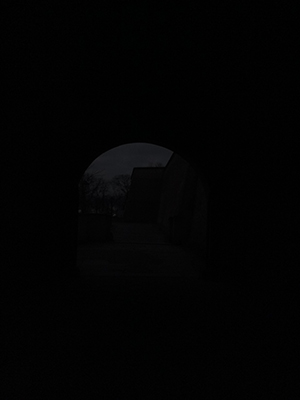
\includegraphics[width=0.08\textwidth]{figures/capturing/series/s0}
	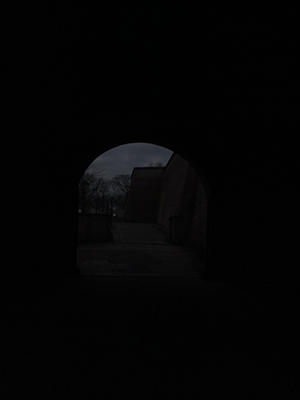
\includegraphics[width=0.08\textwidth]{figures/capturing/series/s1}
	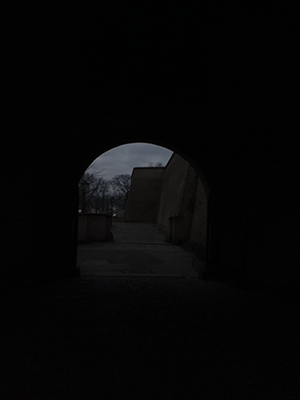
\includegraphics[width=0.08\textwidth]{figures/capturing/series/s2}
	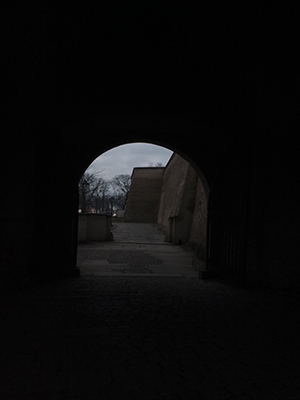
\includegraphics[width=0.08\textwidth]{figures/capturing/series/s3}
	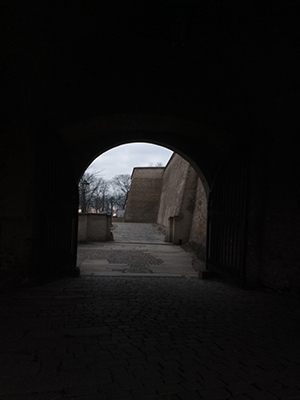
\includegraphics[width=0.08\textwidth]{figures/capturing/series/s4}
	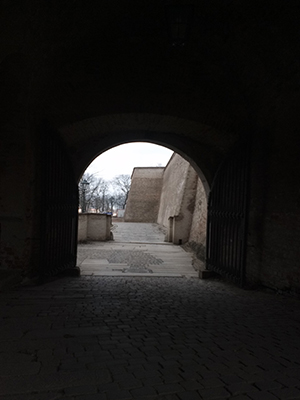
\includegraphics[width=0.08\textwidth]{figures/capturing/series/s5}
	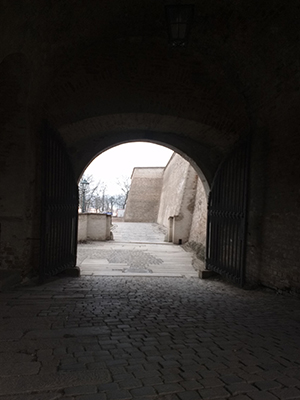
\includegraphics[width=0.08\textwidth]{figures/capturing/series/s6}
	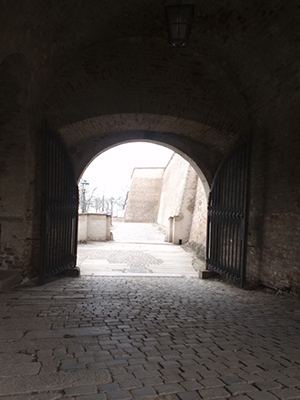
\includegraphics[width=0.08\textwidth]{figures/capturing/series/s7}
	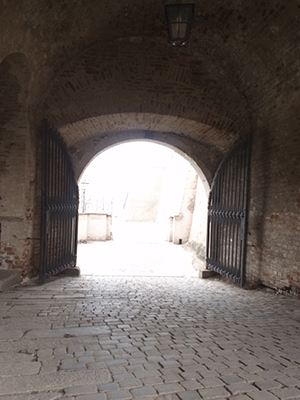
\includegraphics[width=0.08\textwidth]{figures/capturing/series/s8}
	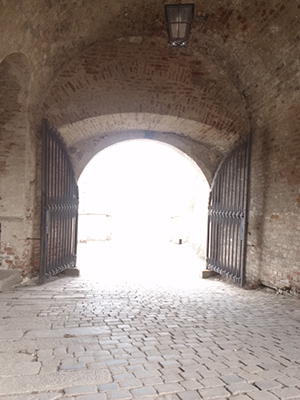
\includegraphics[width=0.08\textwidth]{figures/capturing/series/s9}
	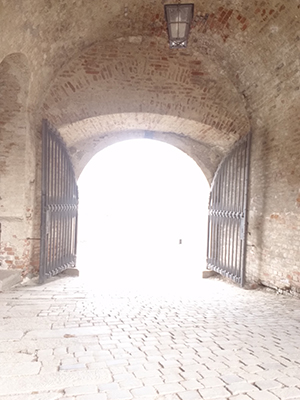
\includegraphics[width=0.08\textwidth]{figures/capturing/series/s10}
  \caption{Séria 11 snímok scény \textit{brana} zachytených s rôznym expozičným časom}
  \label{fig:BranaSeries}
\end{figure}

Pre vytváranie aplikácie, snímanie fotografií scén a záverečné testovanie je použitý tablet SHIELD NVIDIA s operačným
systémom Android 7.0 Nougat. Fotoaparát tabletu má rozlíšenie 5 Mpx a vytvorené snímky rozmer $1944\times2592$ px.
Z pohľadu užívateľa sú bežné fotografie vytvárané týmto zariadením uspokojivé, ale nie dokonalé. Digitálny snímač
nedokáže obsiahnúť taký rozsah farieb a jasu ako štandardný optický fotoaparát. Rozsah expozičného času snímača
tabletu je od 33 600 $ns$ do 356 732 928 $ns$.